\section{Theorie}
\subsection{Das Geiger-Müller-Zählrohr}
Das hier schematisch abgebildete Geiger-Müller-Zählrohr (Abbildung \ref{fig:Querschnitt}) setzt sich zusammen aus einem Kathodenzylinder, der mit einem Gasgemisch gefüllt ist und einem Anodendraht.
\begin{figure}[H]
\begin{center}
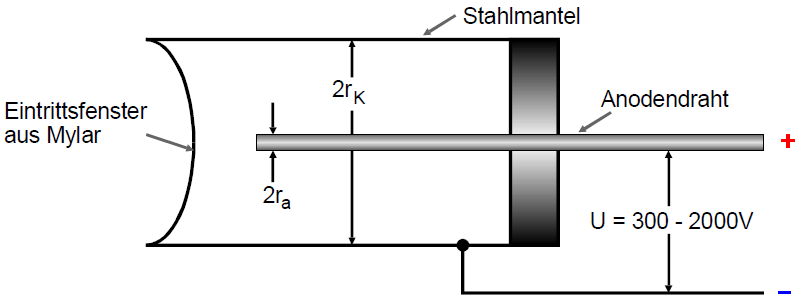
\includegraphics[width = 10cm, height= 4cm]{Querschnitt.png}
\caption{Der Querschnitt durch ein Endfenster-Zählröhrs, welches mit einem Gasgemisch gefüllt ist. Der Anodendraht führt axial durch.\protect\cite{AL}}
\end{center}
\label{fig:Querschnitt}
\end{figure}
\noindent
Das Gasgemisch besteht aus 100 mbar des Edelgases Argon und 10 mbar Ethylalkohol.
Mithilfe des Gases werden Elektronen freigesetzt, die durch die ionisierte Strahlung mit den Atomen des Edelgases zusammenstoßen.
Innerhalb des elektrischen Feldes wandern die freigesetzten Elektronen zur Anode.
Die Öffnung des Zählrohrs ist mit einer Mylar-Folie bedeckt.
Die Folie ist so dünn, dass sie bereits von $\alpha$-Teilchen durchdrungen werden kann.
Der Unterdruck sorgt dafür, dass die Folie eine nach innen gerichtete Wölbung besitzt.
Mit der Anlegung der äußeren Spannung von ungefähr 300-2000 Volt wird ein radialsymmetrisches elektrisches Feld zwischen Kathode und Anode erzeugt,
welches beschrieben wird durch
\begin{align}
    {E}({r}) = \frac{{U}}{{r} \ \text{ln}(\frac{{r}_{{k}}}{{r}_{{a}}})}
\end{align}
Hier entspricht $r$ dem Abstand der Quelle zur Zählrohrachse, $U$ gibt die Spannung an, $r_{(k)}$ bezeichnet den Radius des Kathodenzylinders und
$r_{(a)}$ den des Anodendrahtes.
Das Verhältnis zwischen beiden Radien wird durch
\begin{align}
  {r}_{{a}} < {r} < {r}_{{k}}
\end{align}
bestimmt.
Wenn ein geladenes Teilchen in das Zählrohr gelangt, bewegt es sich solange innerhalb des Gasraumes bis seine Energie durch Ionisationsprozesse aufgebraucht ist.
Die Beschleunigung der eingetretenen Teilchen verhält sich proportional zu $\frac{1}{{r}}$.
Wenn die Zählrohrspannung variiert wird, können fünf unterschiedliche Bereiche des Ablaufs unterschieden werden.
Die Verteilung wird in Abbildung \ref{fig:Zählrohrcharakteristik} dargestellt.
\begin{figure}[H]
\begin{center}
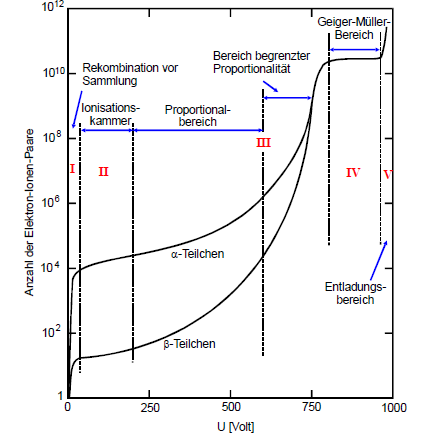
\includegraphics[width = 10cm, height= 9cm]{Zählrohrcharakteristik.png}
\caption{Die Anzahl der erzeugten Elektron-Ionenpaare als Funktion der Spannung U bei einem Proportionazählrohr.\protect\cite{AL}}
\label{fig:Zählrohrcharakteristik}
\end{center}
\end{figure}
\subsection{Erläuterung der Bereiche}
\begin{enumerate}
  \renewcommand{\labelenumi}{\roman{enumi}}
  \item Rekombination
  Im ersten Bereich, der Rekombination, werden nur geringe Ionisationsprodukte an der Anode gemessen.
  Bei niedriger Zählrohrspannung rekombinieren die Teilchen häufig wieder. \\
  \item Ionisationskammer
  Den zweiten Bereich bildet die Ionisationskammer.
  In diesem Bereich steigt die Feldstärke, die Rekombination sinkt und viele Elektronen erreichen die Anode.
  Der Ionisationsstrom stellt sich proportional ein. \\
  \item Proportionalitätsbereich
  Bei Erhöhung der Spannung bildet sich der Proportionalitätsbereich.
  Die freigesetzten Elektronen verfügen über die Potenz Ionisationsvorgänge auszulösen.
  Es entsteht die sogenannte Townsend-Lawine bei der Elektronen, aufgrund der Zusammenstöße andere Elektronen zur Ionisation anregen. \\
  \item Geiger-Müller-Bereich
  Im vierten Abschnitt, dem Geiger-Müller-Bereich, entstehen bei hohen Energien Elektronen und auch hochenergetische UV-Photonen.
  Gleichfalls entstehen Sekundärelektronen, die aus der metallischen Oberfläche des GMZ stammen.
  Es kommt zur Entstehung von Elektronenlawinen, was zum Verlust der Proportionalität zwischen der Ladung und der Teilchenenergie führt.
  Im Bereich vier wird ausschließlich die Intensitätsmessung der Strahlung durchgeführt. \\
  \item Entladungsbereich
  Als letzter Bereich gilt der Entladungsbereich.
  Hier wird die Spannung erhöht (in der Theorie 960 \ ${V}$ - 100 \ ${V}$).
  Die Zahl der Nachentladungen steigt schlagartig.
\end{enumerate}
\subsection{Die Totzeit und die Nachentladung}
Die Totzeit $T$ und Erholungszeit $T_{{E}}$ werden in Abbildung \ref{fig:Zählrohrspannung} dargestellt.
\begin{figure}[H]
\begin{center}
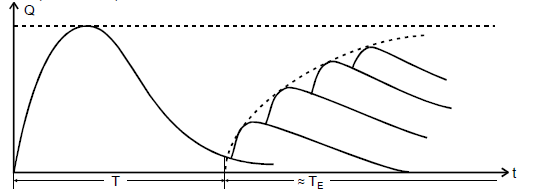
\includegraphics[width = 9cm, height= 5cm]{Zählrohrspannung.png}
\caption{Totzeit $T$ und Erholungszeit $T_{{E}}$ mit Nachentladungen.\protect\cite{AL}}  
\label{fig:Zählrohrspannung}
\end{center}
\end{figure}
\noindent
Unter Totzeit $T$ wird die Zeit verstanden, in der die einfallenden Teilchen die Kathode nicht erreichen.
Die trägen positiven Ionen halten sich im Gasgemisch auf und bilden einen radialsymmetrischen Ionenschlauch.
Dadurch wird die elektrische Feldstärke an der Kathode in Nähe des Drahtes gemindert.
Die Elektronen fließen beim Entladevorgang schnell ab. \\
Die Erholungszeit $T_{{E}}$ beschreibt die Zeit, die benötigt wird, um alle Ionen zu neutralisieren ,bzw. bis alle Ionen abgewandelt sind,
 und einen raumladungsfreien Zustand herzustellen.
Die Ladungsimpulse nehmen ihre Ausgangsamplitude an. \\
Zusätzliche elektrische Impulse werden in der Nachentladung neutralisiert. Die Sekundärelektronen erzeugen den negativen Effekt der Nachentladung.
In dem Gasgemisch wird die Nachentladung unterdrückt.
Die Ionisationsenergien sind zu gering um Moleküle zu ionisieren.
Durch das Hinzufügen von Ethylalkohol in das Zählrohr wird eine Kollision der Edelgasionen mit den
Alhokolionen provoziert.
Eine Kollision mit dem Mantelmaterial findet weniger bis gar nicht mehr statt.
So werden keine Elektronen aus dem Mantel gelöst.
Die Ethylalkoholionen werden durch die Energieaufnahme in Schwingung versetzt, sodass keine Nachentladung stattfinden kann.
\subsection{Charakteristik des Zählrohrs}
Zunächst wird die Charakteristik des Zählrohrs in einer Kurve bei konstanter Intensität in Abbildung \ref{fig:Erholungszeit} dargestellt.
\begin{figure}[H]
\begin{center}
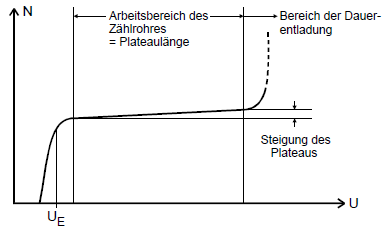
\includegraphics[width = 10cm, height= 6cm]{Erholungszeit.png}
\caption{Charakteristik des GMZs bei konstanter Intensität.\protect\cite{AL}}
\label{fig:Erholungszeit}
\end{center}
\end{figure}
\noindent
Die Pulsrate $N$ wird dabei als Funktion der Spannung $U$ beschrieben.
Bei $U_{{E}}$ beginnt der Auslösebereich. Im Anschluss zeigt sich ein linearer Bereich, der den Plateauabschnitt kennzeichnet.
Im Idealfall besitz das Zählrohr eine Steigung des Plateaus von Null.
In der Praxis ergibt sich jedoch eine geringe Steigung, Grund dafür sind die Nachentladungen.
Die Qualität des Zählrohres und die Abbildung des Plateaubereiches charakterisieren die Güte des Experiments.
Der Zusammenhang bildet sich je kleiner die Steigung und je länger der Plateaubereich ist, desto hochwertiger ist das Zählrohr.
Nach dem Plateau tritt der Bereich der Dauerentladung ein und die Nachentladung steigt stark an.
\label{sec:Theorie}


